% !TEX encoding = UTF-8 Unicode
%!TEX root = main.tex
% !TEX spellcheck = en-US
%%=========================================


%%%%%%%%%%%%%%%%%%%%%%%%%%%%%%%%%%%%%%%%%%%%%%%%%%%%%%%%%%%%%%%%%%%%%%%%%%%%%%%%%%%
\chapter{Design}
\label{ch:design}


First of all, ProXC++ is a concurrency library for C++. Only recently as of C++11 has the C++ programming language added concurrency primitives to the standard library, such as threading and futures. However, C++ lacks any standard support for concurrency in user space. 

Designing a concurrency library for C++ with dynamic multithreading requires some notion of user space threading mechanism, which in turn requires a runtime system. This runtime system acts as an invisible layer between the program and the operating system, handling resources and logistics of scheduling the different processes running in the program. 

All library functionality, such as channels, builds upon the framework provided by the runtime system. Essentially, anything must be done via the runtime system, which is why the limitations of the runtime system functionality limits the potentiality of the library functionality.

This chapter contains a full design of ProXC++, and explains some of the design choices. The runtime system is first designed, and subsequently the library features are designed based on the runtime system functionality. 


%%%%%%%%%%%%%%%%%%%%%%%%%%%%%%%%%%%%%%%%%%%%%%%%%%%%%%%%%%%%%%%%%%%%%%%%%%%%%%%%
\section{Runtime System}


Before discussing the design of the runtime system, lets first identify what the responsibilities of the runtime system are. A ProXC++ program contains a set of processes, where each process represents some point of execution. The runtime system must be able to spawn, schedule, and synchronize these processes, i.e. process management. A scheduler could therefore be responsible for process management. 

For a singlecore runtime system, only a single scheduler makes sense. However, how many schedulers are optimal for a dynamic multithreaded runtime system? Given the maximum number of parallel executions on a processor is equal to the number of available processor cores, the optimal number of schedulers is the number of available processor cores, and each scheduler runs on its own processor core. If more schedulers where online than available processor cores, situations would occur were multiple schedulers are struggling to run on the same processor core, which would be unproductive.

Another important factor is how process management is shared among schedulers. Two principal strategies exists, namely \textit{centralized} or \textit{distributed} management. Given a centralized management, all schedulers share the same control structures, including a shared process queue for which processes are to be scheduled from. All schedulers share the responsibility for all processes in a program. Given a distributed management, all schedulers has a set of processes for which it has the responsibility of managing. Schedulers share nothing, essentially meaning all processes has a parent scheduler.

A centralized management is easy to implement, as the entire runtime system such as control structures and processes  is shared between schedulers. Schedulers does not have to worry about distributing processes for scheduling, as all processes are scheduled through the same queue. However, it does not scale as well with an increase in processor cores, as it creates contention between the increase in schedulers accessing the shared control structures. Distributed management is much harder to implement, as now each scheduler has its own set of control structures and processes. The main issue is how to efficiently distribute ready processes between schedulers. If done right, distributed management scales very well with an increase in processor cores.

Given that ProXC++ aims to be a high\hyp{}performance concurrency library, distributed process management is necessary for catering to all multicore architectures.

To summarize, the runtime systems consists of a number of schedulers equal to the number of available processor cores. Process management is distributed among the schedulers, meaning each scheduler has responsibility of a set of processes.


%%%%%%%%%%%%%%%%%%%%%%%%%%%%%%%%%%%%%%%%
\subsection{Scheduler}


The scheduler is the core of the runtime system, providing the logic and control structures necessary for process management. Given a scheduler, a set of zero\hyp{}or\hyp{}more unique processes are said to be under the schedulers management. This scheduler is the \textit{parent scheduler} of said processes, which are called \textit{work processes}.

A scheduler is either \textit{running} or \textit{idle}. A running scheduler has one\hyp{}or\hyp{}more work processes which are ready to be scheduled for execution, or simply called ready. When the scheduler runs out of ready work processes, it becomes idle.

Ready work processes are stored in a process queue called the \textit{ready queue}. The scheduler uses the ready queue to determine whether it has ready work processes or not, i.e. an idle scheduler has an empty ready queue. When a scheduler has a non\hyp{}empty ready queue, a work process is removed from the ready queue and resumed execution. Scheduling and rescheduling a work process is equivalent with adding the process to the ready queue.

As processes are scheduled in user space, the scheduler relies on \textit{cooperative scheduling}. Cooperative scheduling entails running processes voluntarily yielding running time to the scheduler. If a processes never yields to the scheduler, the process will run for ever. 

The main challenge of the scheduler is how to distribute superfluous ready work processes to schedulers which are idle. Two principal strategies exist: \textit{work sharing} and \textit{work stealing}. Work sharing consists of manually distributing new work processes among the schedulers. Work stealing consists of stealing ready work from other schedulers when a scheduler runs out of ready work, i.e. becoming idle. 

Work stealing is usually preferred over work sharing as it causes less process migration. Process migration is when management responsibility of a process is transferred between schedulers, or in other words the process changes its parent scheduler. Work stealing is however more complex to implement than work sharing, but scales much better on distributed multiprogrammed systems. Therefore, work stealing is employed as the load distribution strategy for the schedulers.


%%%%%%%%%%%%%%%%%%%%%%%%%%%%%%%%%%%%%%%%
\subsection{Processes}


Processes represent some point of execution. As stated above, all work processes has a parent scheduler which corresponds to the scheduler running on a particular processor core. A scheduler is also a process but differs from work processes, as a work process represents meaningful work from the running program. 

A work process with a corresponding parent scheduler may spawn new work processes. These new processes are scheduled by the parent scheduler. A work process may also synchronize or join on other work processes, meaning waiting for the other work process to terminate. 

Some work processes may suspend itself, waiting for other work processes to reschedule the suspended process. The suspending work process simply yields to the scheduler. Suspended processes are not stored in any queues, as other work processes will reschedule the suspended process rather than the scheduler. 

Work processes may also suspend, or sleep, until a given or derived time point. These processes are added to the parent schedulers \textit{sleep queue}. The parent scheduler will frequently examine the sleep queue and reschedule any work processes with an expired time point. If a work process sleeps but is rescheduled by another work process before the time point is expired, the scheduler will reschedule and remove the waking process from the sleep queue.


%%%%%%%%%%%%%%%%%%%%%%%%%%%%%%%%%%%%%%%%%%%%%%%%%%%%%%%%%%%%%%%%%%%%%%%%%%%%%%%%
\section{Feature Design}




%%%%%%%%%%%%%%%%%%%%%%%%%%%%%%%%%%%%%%%%
\subsection{Timers}
\label{subsec:timers_desgin}


Three types of timers are available: \textit{egg}, \textit{repeat} and \textit{date} timer. Timers are used for either explicit process suspension, or for timeout on channel or alternation operations. 

Egg timer is used for relative timeout. Just as an egg timer in real life, it is used to countdown for a specified period of time. It is not a one\hyp{}shot timer, meaning the same timer can be reused multiple times. The countdown begins at the start of an operation, effectively resetting the timer if already used.

Repeat (or loop) timer is used for a periodic repeating timeout. The repeat timer will timeout in a periodic fashion, given a specified period of time. The timer only resets after timeout. Compared to the egg timer, the repeat timer is also not a one\hyp{}shot timer and can be reused, but the repeat timer does not reset the countdown at the start of an operation.

Date timer is used for absolute timeout. It is a one\hyp{}shot timer, and will always be expired after timeout. The date timer timeouts at a specified time point. The timer can never be reset, and therefore survives multiple operations.


%%%%%%%%%%%%%%%%%%%%%%%%%%%%%%%%%%%%%%%%
\subsection{Fork\hyp{}Join Parallelism}
\label{subsec:fork_join_parallelism}


Processes can spawn new processes in parallel with the \textit{parallel} statement. The parallel statement takes one or more processes, either as single process statements or process replicators, and spawns and runs these processes in parallel. The spawned processes runs concurrently with any other processes currently running in the program. The parallel statement is the only way to spawn new processes with ProXC++.

The parallel statement follows the fork\hyp{}join model \citep[page 88]{mccool2012structured}, where a sequential execution branches off at a designated point into parallel work, and subsequently joins/merges at another designated point and resumes the original sequential execution. \Cref{fig:fork_join_model} gives a simple illustration of the fork\hyp{}join model.

\begin{figure}[h!]
    \centering
    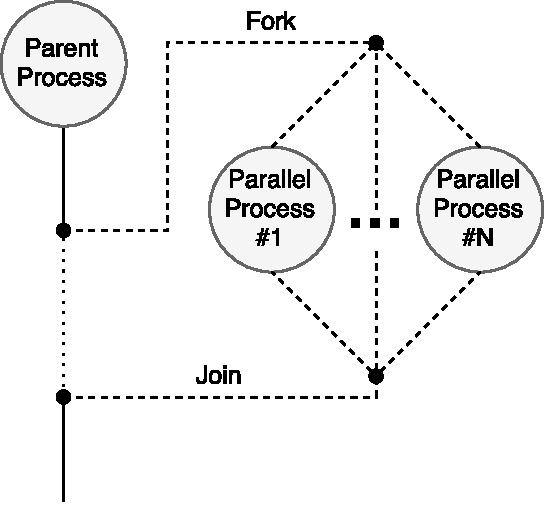
\includegraphics[width=0.6\linewidth]{fig/fork_join}
    \caption{A parent process spawns $N$ parallel processes following the fork\hyp{}join model.}
    \label{fig:fork_join_model}
\end{figure}

The process calling the parallel statement is the parent process. When calling the parallel statement, the parent process is suspended until all processes within the parallel statement has spawned, executed and terminated. When all parallel processes has terminated, the parent process resumes execution. 

The processes to be executed in parallel can be defined in two ways: either as a single process or as a replicated process. See \cref{subsec:processes} for a more detailed explanation of processes. 

%%%%%%%%%%%%%%%%%%%%%%%%%%%%%%%%%%%%%%%%
\subsection{Channels}
\label{subsec:channel_design}


Channels forms the only means of communication as well as synchronization between work processes via message\hyp{}passing. Given a channel, some type of message can be transmitted between a sender and a receiver.

Hereafter, the term ``\textit{Tx}'' denotes a channel end for which a work process is sending on, and the term ``\textit{Rx}'' denotes a channel end for which a work process is receiving on. The term ``\textit{participant}'' denotes either a Tx or Rx.

An synchronous channel implies both a Tx and a Rx must be at a channel to complete a channel operation, e.g. a Tx cannot transmit a message without a Rx ready to receive. If only one of the two required participants are ready to transmit, the participant must block (wait) until the other side is ready. This kind of behaviour is called \textit{rendezvous}. A synchronous channel is also unbuffered, given that no messages are stored intermediately in the channel.

The opposite of a synchronous, unbuffered channels are asynchronous, buffered channels, where messages are buffered if there are no receivers ready. Tx never waits regardless of a ready Rx or not, while Rx must only wait if the buffer is empty. See \cref{fig:channel_sync_async} for an illustration of the difference between synchronous and asynchronous channels.

\begin{figure}[h!]
    \centering
    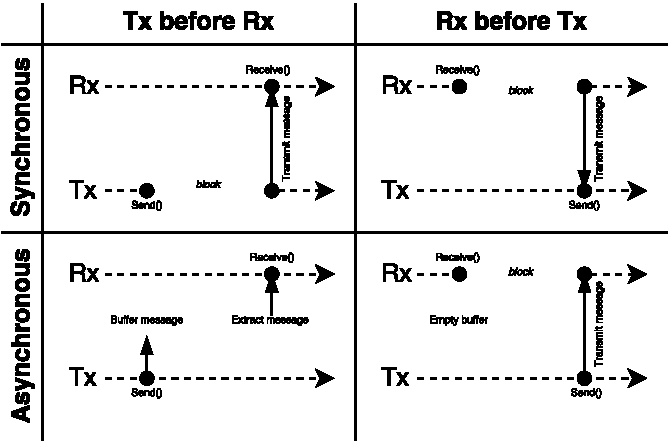
\includegraphics[width=1\linewidth]{fig/channel_sync_async}
    \caption{Different configurations of synchronous and asynchronous channel communication.}
    \label{fig:channel_sync_async}
\end{figure}

Synchronous channels are usually preferred over asynchronous channels, as it is more deterministic. When a channel operation is completed, both participants know the opposite participant is in a particular state. This is not the case for asynchronous channels. Regarding memory use, synchronous channels always require constant memory while asynchronous channels has to allocate memory for its buffer.

A unidirectional channel only allows messages to be transmitted in one direction. In contrast, a bidirectional channel allows messages to be transmitted in both directions. Unidirectional channels are more restrictive than bidirectional channels. The argument for unidirectional channels is for bidirectional channel it is possible for both participants to disagree which direction a channel transmission is. The direction of a channel transmission for a unidirectional channel is always given.

Some channel design has the concept of limiting how many unique processes can access and use a channel. This concept is called \textit{disjointness rules} in XC \citep{douglas2009programming} and \textit{usage rules} in occam \citep{barrett1992occam}. In essence, these ``rules'' specify if either end of a channel, sending and receiving, can only be used by a unique process or any processes. Usually denoted by \textit{one/any\hyp{}to\hyp{}one/any}, this gives the four configurations: \textit{one\hyp{}to\hyp{}one}, \textit{one\hyp{}to\hyp{}any}, \textit{any\hyp{}to\hyp{}one}, and \textit{any\hyp{}to\hyp{}any}. Both XC and occam follows the one\hyp{}to\hyp{}one design.

Ensuring both Tx and Rx agrees on the type of message being transmitted has to do with \textit{type safety}. If both participants of a channel operations disagrees in the type of the transmitted message, a \textit{type error} occurs. Type safety is therefore to discourage or prevent type errors. It is obviously desirable for a type safe channel, but it is highly dependent on support from either the programming language or the compiler to enforce type safety. A compromise is size safe channels, where both participants agree on the size of the message rather than the type. Size safety is not as desirable as type safety, but is much more doable to enforce.

Channels has a notion of being open or closed. An open channel operates as normal, but a closed channel will deny any operations being completed. A channel always starts as open, and can be closed in on of two ways: an explicit close from either participant, or one of two channel ends goes out of scope, i.e. is no longer available. When a channel becomes closed it remains closed. A closed channel is used to signal participants when no more values will be sent on the channel, which is useful to communicate completion to the opposite channel end.

Considering the different channel factors above, channels in ProXC++ are synchronous and unbuffered, unidrectional, one\hyp{}to\hyp{}one and type safe.


%%%%%%%%%%%%%%%%%%%%%%%%%%%%%%%%%%%%%%%%
\subsection{Alting}
\label{subsec:alting_design}


Alternation is a construct allowing to wait on multiple alternatives simultaneously, selecting an alternative when one or more alternatives are ready. Each alternative has an optional corresponding block of code (closure) which is executed if chosen. Alternatives can also be guarded by a boolean value, enabling or disabling certain alternatives on certain conditions. These boolean guards are evaluated at the initialization of the alternation procedure.

Three types of alternatives exists: channel operations, timers, and skip. Channel operation alternatives include both sending and receiving.

The alternation procedure works as follows: at initialization, zero or more alternatives are enabled for selection. Each enabled alternative is checked if ready to synchronize. If one or more alternatives are ready, one is selected. If none are ready, the alternation procedure suspends and waits for the first alternative to become ready. This first ready alternative is automatically selected. When the alternation procedure has selected an alternative, the corresponding closure is executed if present.

The alternatives operates, when enabled, as follows:

\begin{enumerate}[topsep=0em,itemsep=-1em,partopsep=0.5em,parsep=1em]
    \item \textbf{Channel operation} -- specifies a channel send or receive. A channel send is accompanied with the item to transmit, while a channel receive can optionally capture the received item in the alternative closure. The alternative becomes ready when the opposite side of the channel operation is present.
    \item \textbf{Timeout} -- is a timer with a corresponding timeout. If the alternation process has not selected an alternative before timeout, the timer alternative is selected.
    \item \textbf{Skip} -- is an alternative which is always ready. It can be compared to the \texttt{default} case in switch cases. If no alternatives are ready at the alternation initialization, the skip alternative is selected. 
\end{enumerate}

Multiple channel alternatives can be enabled for an alternation procedure. Multiple timer alternatives can also be enabled for an alternation procedure, however only the timer with the shortest deadline will be registered. If multiple skip alternatives are enabled, only the first skip alternative is registered.

An channel alternative can either be selected \textit{actively} or \textit{passively}. Actively selecting involves the alternation procedure performing the selection, while passively selecting involves external events performing the selection. A channel alternative can also only be selected after being entered. Entering a channel alternative is essentially registering the interest of the alternation procedure to perform the channel operation. Leaving a channel alternative performs the opposite, unregistering this interest.



%%%%%%%%%%%%%%%%%%%%%%%%%%%%%%%%%%%%%%%%%%%%%%%%%%%%%%%%%%%%%%%%%%%%%%%%%%%%%%%%
\section{Runtime Algorithms}


%%%%%%%%%%%%%%%%%%%%%%%%%%%%%%%%%%%%%%%%
\subsection{Work Stealing Algorithm}
\label{subsec:work_stealing_algorithm}


As each scheduler has their unique set of work processes, work stealing is employed to distribute superfluous work processes from a running scheduler to an idle scheduler. 

The work stealing algorithm centers around the ready queue. As long as the scheduler has work processes in its ready queue, the scheduler will continue to resume work processes from the queue. However, when the ready queue becomes empty, the scheduler resort to work stealing. Work stealing goes as follows:

\begin{enumeratefloat}
\begin{enumerate}[topsep=0em,itemsep=-1em,partopsep=0.5em,parsep=1em]
    \item \textbf{Select victim} -- another scheduler, called a victim, is randomly chosen.
    \item \textbf{Try stealing} -- the current scheduler tries to steal some work processes from the victim. If failed, restart procedure;
    \item \textbf{Resume work} -- else, the stolen work processes are stored in the ready queue, and a work process is resumed.
\end{enumerate}    
\caption{Observations for both non\hyp{}alting and alting channel ends.}
    \label{list:conjecture_both}
\end{enumeratefloat}

As simple as the algorithm sounds, some details must be taken into consideration. Is it feasible for an idle scheduler to repeatedly retrying to steal work until it succeeds? Stealing a process is the same as process migration, and process migration does cause some overhead. Consider the following programs which has a few number of parallel processes or many dependent processes. An aggressive work stealing scheme would cause many unnecessary process migrations, compared to none for a singlecore runtime system. 

To mitigate unnecessary process migrations by overaggressive work stealing, an idle scheduler can either wait for a short period of time before retrying, or it could wait until signaled by a scheduler with superfluous work processes. 


%%%%%%%%%%%%%%%%%%%%%%%%%%%%%%%%%%%%%%%%
\subsection{Channel End Algorithm}
\label{subsec:channel_end_algorithm}


The channel algorithm is different whether the channel end is alting or not. A set of observations are postulated in \cref{list:conjecture_both,list:conjecture_nonalting,list:conjecture_alting} to form the basis of the channel algorithm.

\FloatBarrier

\begin{enumeratefloat}
    \begin{enumerate}[topsep=0em,itemsep=-1em,partopsep=0.5em,parsep=1em]
        \item A channel operation consists of a single Tx and a single Rx arriving in either sequential order, both of which can be alting or non\hyp{}alting.
        \item When a channel end has arrived for a channel operation, another channel end of same type cannot arrive before that channel operation has completed.
        \item Any channel end may at most suspend once during a channel operation.
        \item The last channel end to arrive at a channel operation will always complete the item transmission.
        \item If a channel end is suspended during a non\hyp{}timed channel operation, it is only rescheduled if the channel operation completed or the channel closed.
        \item During a timed channel operation, a suspended channel end may also be rescheduled if a timeout occurs.
    \end{enumerate}
    \caption{Observations for both non\hyp{}alting and alting channel ends.}
    \label{list:conjecture_both}
\end{enumeratefloat}

\begin{enumeratefloat}
    \begin{enumerate}[topsep=0em,itemsep=-1em,partopsep=0.5em,parsep=1em]
        \item The non\hyp{}alting channel end arriving first at an channel operation will always suspend.
        \item The channel end arriving last at an channel operation will never suspend.
        \item A process holding both channel ends for a channel will always block indefinitely if operating on the given channel.
        \item A channel end never leaves the channel operation after arrival unless it completes, the channel closes, or times out, i.e. a channel end always commits to a channel operation.
    \end{enumerate}
    \caption{Observations for non\hyp{}alting channel ends.}
    \label{list:conjecture_nonalting}
\end{enumeratefloat}

\begin{enumeratefloat}
    \begin{enumerate}[topsep=0em,itemsep=-1em,partopsep=0.5em,parsep=1em]
        \item A channel end never explicitly suspends during a channel operation. This is done indirectly by the alting procedure.
        \item A channel end may leave the channel operation after arrival and return later, i.e. a channel end may not commit to a channel operation.
    \end{enumerate}
    \caption{Observations for alting channel ends.}
    \label{list:conjecture_alting}
\end{enumeratefloat}

\FloatBarrier

A key observation to make from the observations in \cref{list:conjecture_both,list:conjecture_nonalting,list:conjecture_alting} is the symmetry of the channel operation; it is invariant whether Tx or Rx is completing the operation. This makes the algorithm very much the same for both sending and receiving on a channel. Another observation to make is how non\hyp{}alting channel ends commit, while alting channel ends may not commit. This skew in committal channel ends allows for important assumptions in the algorithm.


%%%%%%%%%%%%%%%%%%%%%%%%%%%%%%%%%%%%%%%%
\subsubsection{Non\hyp{}Alting Channel End Algorithm}

A non\hyp{}alting channel end has two cases to consider: either the other channel end is non\hyp{}alting or alting. 
A channel operation for a non\hyp{}alting channel end can be considered to consists of three possible steps:

\begin{enumerate}[topsep=0em,itemsep=-1em,partopsep=0.5em,parsep=1em]
    \item \textbf{Check channel is open} -- return if the channel is closed, else continue.
    \item \textbf{Check for opposite channel end} -- if an opposite channel end is present at the channel, try selecting the channel end. If successful, complete the transmission, reschedule opposite channel end and return ok. Else, continue.
    \label{step:channel_nonalt_complete}
    \item \textbf{Wait for opposite channel end} -- register the channel end in the channel and suspend. When rescheduled, check if the item was transmitted or not and return appropriately.
    \label{step:channel_nonalt_wait}
\end{enumerate}

Note that the entire procedure is surrounded by mutual exclusion using the channel lock, because the channel ends must arrive at the channel in a sequential order.

To elaborate on step \ref{step:channel_nonalt_complete}, selecting the opposite channel end is necessary since an alting opposite channel end is not committal to the channel operation, even though it is present. Selecting a non\hyp{}alting channel end is always successful since it is always committal, while an alting channel end may fail. This selection process is further explained in \cref{sec:alternation}.

Completing the transmission in step \ref{step:channel_nonalt_complete} involves transmitting the item and setting the consumed flag, and checking the transmission in step \ref{step:channel_nonalt_wait} involves checking and resetting the consumed flag.

The consumed flag is necessary to signal the suspended channel end if the item was transmitted, even though the channel has been closed. Consider this situation: Tx enters the channel and is suspended, waiting for an Rx. Rx enters the channel, completes the transmission, and reschedules Tx. Before Tx is resumes execution, Rx closes the channel. Now, when Tx resumes it is impossible to tell if Tx was rescheduled because of completed operation or channel closing. The consumed flag is here to signal the rescheduled channel end was rescheduled because of either case.


%%%%%%%%%%%%%%%%%%%%%%%%%%%%%%%%%%%%%%%%
\subsubsection{Alting Channel End Algorithm}

An alting channel end also has two cases to consider: either the other channel end is non\hyp{}alting or alting. The non\hyp{}alting case is trivial, because if the opposite end is present then simply complete the transmission. The alting case is however more complicated. 

Before describing the algorithm, first consider this situation: Two processes both alting on the same two channels, however each process have the Tx of one channel and Rx of the other, making a cycle. See \cref{fig:alting_problem} for illustration. Both of these alting processes must somehow agree on which case they both select. Some sort of synchronization between two alting channel ends must therefore exist. Note that this alt\hyp{}to\hyp{}alt synchronization must be asymmetrical to avoid deadlocks.

\begin{figure}[h!]
    \centering
    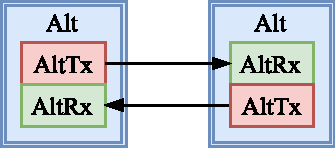
\includegraphics[width=0.6\linewidth]{fig/alting_problem}
    \caption{Illustration of the cyclic alting problem.}
    \label{fig:alting_problem}
\end{figure}

A value with three possible states is used for alt\hyp{}to\hyp{}alt synchronization. The three states are \textit{none}, \textit{offered}, and \textit{accepted}. Given all alting channel ends have a well defined static ordering, the alt\hyp{}to\hyp{}alt synchronization protocol says the lower ranked channel end is to offer synchronization, while the higher ranked channel end is to accept. Note that for this to not be symmetric, the ordering must be invariant of the channel end type.

Given this alt\hyp{}to\hyp{}alt synchronization, the alting channel end algorithm is as follows:

\begin{enumerate}[topsep=0em,itemsep=-1em,partopsep=0.5em,parsep=1em]
    \item \textbf{Check alt\hyp{}to\hyp{}alt synchronization} -- if an opposite channel end is present and is alting, check synchronization state. Else, continue. If offered, accept and complete the alt\hyp{}to\hyp{}alt transmission. Else, return and try later.
    \label{step:check_alt_sync}
    \item \textbf{Check channel is open} -- return if the channel is closed, else continue.
    \item \textbf{Check for opposite channel end} -- return if there is no opposite channel end present, else continue.
    \item \textbf{Check if opposite channel end is non\hyp{}alting} -- if the opposite channel is non\hyp{}alting, complete the transmission, reschedule opposite channel end and return ok. Else, continue.
    \label{step:opposite_side_nonalting}
    \item \textbf{Check rank of opposite channel end} -- compare the rank of the opposite channel end with self.
    \item \textbf{Self has lower rank} -- offer synchronization and wait until response. If the sync was accepted, return ok. Else, return appropriately.
    \label{step:self_lower_rank}
    \item \textbf{Self has higher rank} -- check synchronization state. If offered, complete transmission and accept synchronization. Else, return appropriately.
    \label{step:self_higher_rank}
\end{enumerate}

The reason for checking the alt\hyp{}to\hyp{}alt synchronization in step \ref{step:check_alt_sync} before checking the channel is open has to do with acquiring the channel lock. Since the lock is held by the opposite channel end while offering synchronization, an offered synchronization must be resolved before acquiring the channel lock.

In step \ref{step:opposite_side_nonalting} the alting channel end does not need to synchronize with the opposite channel end if it is non\hyp{}alting, due to selecting a non\hyp{}alting channel ends always succeeds. 

The synchronization procedure in step \ref{step:self_lower_rank} is a little more convoluted than stated, since the alt\hyp{}to\hyp{}alt synchronization is only needed if the opposite alting procedure is checking. If it is waiting, normal selection is used.

The synchronization procedure in step \ref{step:self_higher_rank} is more straightforward. If synchronization is offered, complete the transmission and accept. If it is not offered, check the alting procedure state. If the alting procedure state is checking, try later. If the state is waiting, try normal selection. 


%%%%%%%%%%%%%%%%%%%%%%%%%%%%%%%%%%%%%%%%
\subsection{Alting Algorithm}
\label{subsec:alting_algorithm}


The alternation algorithm works in three phases: \textit{checking}, \textit{waiting}, and \textit{completing} phase. The waiting phase is only entered if the checking phase results in no selected alternatives.

\begin{enumerate}[topsep=0em,itemsep=-1em,partopsep=0.5em,parsep=1em]
    \item \textbf{Checking phase} -- is the active phase of the procedure, where alternatives can be actively selected. Each enabled channel alternative is entered. Next, all channel alternatives are checked if ready. If one or more are ready, all ready channel alternatives are actively selected in random order. When the first alternative is successfully selected, the alternation procedure continues to the completing phase. If no channel alternatives are ready or no channel alternatives are successfully selected, the alternation procedure continues to the waiting phase.
    \item \textbf{Waiting phase} -- is the passive phase of the procedure, where alternatives can be passively selected. If a skip alternative is enabled, the skip alternative is now selected and the procedure continues to the completing phase. If a timer alternative is enabled the procedure suspends itself until the timer expires, else the procedure suspends itself indefinitely. When the procedure is rescheduled, it is either because of an channel alternative passively selecting or the timer alternative has expired, and the corresponding alternative is selected.
    \item \textbf{Completing phase} -- each channel alternative which were entered are now left, and the closure of the selected alternative is executed if present. This completes the alternation procedure.
\end{enumerate}

Note that if any channel alternatives becomes ready after it has been checked by the alternation procedure in the checking phase, that alternative has to wait until the procedure enters the waiting phase to try passively select itself.

Given a number of channel alternatives are ready during the checking phase, each alternative must be resolved before continuing to the waiting or completing phase. Resolving a channel alternative involves trying to complete the channel operation, which either results in a success or fail. The first channel alternative which results in a success short\hyp{}circuits the selection order and continues to the completing phase. However, an alt\hyp{}to\hyp{}alt channel operation has a slightly larger overhead because of alt\hyp{}to\hyp{}alt synchronization, which means trying to complete the channel operation may result in a try\hyp{}later result. A try\hyp{}later result means the alt\hyp{}to\hyp{}alt synchronization cannot be resolved right now, and must be tried later. The selection order therefore skips the alternative and tries later. All channel alternatives must be resolved failed before continuing to the waiting phase.



